\subsection{Définition : }
Le modèle relationnel a été introduit pour la première fois par Ted Codd du centre de recherche d’IBM en 1970 dans un papier désormais classique, et attira immédiatement un intérêt considérable en raison de sa simplicité et de ses fondations mathématique.

Dans ce modèle, les données sont représentées par des tables, sans préjuger de la façon dont les informations sont stockées dans la machine. Les tables constituent donc la structure logique du modèle relationnel, d’autre part ces données sont gérées par un système de gestion de bases de données relationnelle (relational database management system, en anglais), qui représente un système intégré pour la gestion unifiée des bases de données relationnelles, il est constitué d’un composant de stockage et d’un composant de gestion de données.

L’interface standard pour une base de données relationnelle est le langage SQL (Structured Query Language) considéré comme le langage de manipulation des données relationnelles le plus utilisé aujourd’hui. Il est devenu un standard de fait pour les SGBD relationnels. Il possède des caractéristiques proches de l’algèbre relationnelle (jointures, opérations ensemblistes) et d’autres proches du calcul des tuples (variables sur les relations). SQL est un langage redondant qui permet souvent d'écrire les requêtes de plusieurs façons différentes.

\begin{figure}[h]
	\centering
    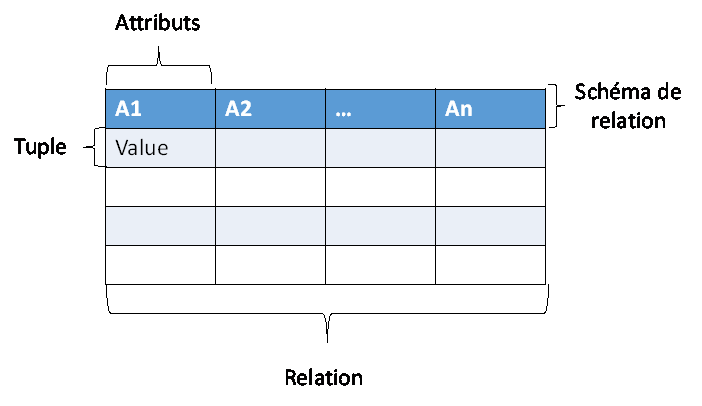
\includegraphics[scale=0.5]{img/4.0.1}
    \caption{Éléments d'une table d'une BDDR.}
\end{figure}